\documentclass[11pt]{article}

%%%%%%%%%%%%%%%%%%%%%%%%%%%%%%%%%%%%%%%%%%%
% Packages                                %
%%%%%%%%%%%%%%%%%%%%%%%%%%%%%%%%%%%%%%%%%%%
\usepackage[margin=1in]{geometry}
\usepackage{color}
\usepackage{xcolor}
\usepackage{amsmath, amsfonts}
\usepackage{enumerate}
\usepackage{graphicx}
\usepackage{titling}
\usepackage{xfrac}
\usepackage{fancyhdr}
\usepackage{natbib}
\usepackage{amsmath}
\usepackage{amssymb}
\usepackage{amsthm}
\usepackage{paralist}
\usepackage{epstopdf}
\usepackage{tabularx}
\usepackage{longtable}
\usepackage{multirow}
\usepackage{multicol}
\usepackage{fancyvrb}
\usepackage{algorithm}
\usepackage{algorithmicx}
\usepackage[noend]{algpseudocode}
\usepackage{float}
\usepackage{xcolor}
\usepackage{array}
\usepackage{times}
\usepackage{url}
\usepackage{comment}
\usepackage{environ}
\usepackage{textcomp}
\usepackage{caption}
\usepackage[colorlinks=true, urlcolor=purple]{hyperref}
\usepackage{cleveref}
\usepackage{parskip} % For NIPS style paragraphs.
\usepackage[compact]{titlesec} % Less whitespace around titles
\usepackage[inline]{enumitem} % For inline enumerate* and itemize*
\usepackage{datetime}
\usepackage{lastpage}
\usepackage[final]{listings}
\usepackage{tikz}
\usetikzlibrary{shapes,decorations}
\usepackage{framed}
\usepackage{booktabs}
\usepackage{cprotect}
\usepackage{verbatimbox}
\usepackage{hyperref}
\usepackage{subcaption}
\usepackage{mathtools} % For drcases
\usepackage{cancel}
\usepackage[many]{tcolorbox}
\usepackage{sectsty}
\usepackage{bm}
\usepackage{nicefrac}

%%%%%%%%%%%%%%%%%%%%%%%%%%%%%%%%%%%%%%%%%%%
% Custom commands are defined within the  %
% common.tex file                         %
%%%%%%%%%%%%%%%%%%%%%%%%%%%%%%%%%%%%%%%%%%%
\input{common.tex}
\def\mA{\mathcal{A}}
\def\mB{\mathcal{B}}
\def\mC{\mathcal{C}}
\def\mD{\mathcal{D}}
\def\mE{\mathcal{E}}
\def\mF{\mathcal{F}}
\def\mG{\mathcal{G}}
\def\mH{\mathcal{H}}
\def\mI{\mathcal{I}}
\def\mJ{\mathcal{J}}
\def\mK{\mathcal{K}}
\def\mL{\mathcal{L}}
\def\mM{\mathcal{M}}
\def\mN{\mathcal{N}}
\def\mO{\mathcal{O}}
\def\mP{\mathcal{P}}
\def\mQ{\mathcal{Q}}
\def\mR{\mathcal{R}}
\def\mS{\mathcal{S}}
\def\mT{\mathcal{T}}
\def\mU{\mathcal{U}}
\def\mV{\mathcal{V}}
\def\mW{\mathcal{W}}
\def\mX{\mathcal{X}}
\def\mY{\mathcal{Y}}
\def\mZ{\mathcal{Z}}

\def\1n{\mathbf{1}_n}
\def\0{\mathbf{0}}
\def\1{\mathbf{1}}


\def\A{{\bf A}}
\def\B{{\bf B}}
\def\C{{\bf C}}
\def\D{{\bf D}}
\def\E{{\bf E}}
\def\F{{\bf F}}
\def\G{{\bf G}}
\def\H{{\bf H}}
\def\I{{\bf I}}
\def\J{{\bf J}}
\def\K{{\bf K}}
\def\L{{\bf L}}
\def\M{{\bf M}}
\def\N{{\bf N}}
\def\O{{\bf O}}
\def\P{{\bf P}}
\def\Q{{\bf Q}}
\def\R{{\bf R}}
\def\S{{\bf S}}
\def\T{{\bf T}}
\def\U{{\bf U}}
\def\V{{\bf V}}
\def\W{{\bf W}}
\def\X{{\bf X}}
\def\Y{{\bf Y}}
\def\Z{{\bf Z}}

\def\a{{\bf a}}
\def\b{{\bf b}}
\def\c{{\bf c}}
\def\d{{\bf d}}
\def\e{{\bf e}}
\def\f{{\bf f}}
\def\g{{\bf g}}
\def\h{{\bf h}}
\def\i{{\bf i}}
\def\j{{\bf j}}
\def\k{{\bf k}}
\def\l{{\bf l}}
\def\m{{\bf m}}
\def\n{{\bf n}}
\def\o{{\bf o}}
\def\p{{\bf p}}
\def\q{{\bf q}}
\def\r{{\bf r}}
\def\s{{\bf s}}
\def\t{{\bf t}}
\def\u{{\bf u}}
\def\v{{\bf v}}
\def\w{{\bf w}}
\def\x{{\bf x}}
\def\y{{\bf y}}
\def\z{{\bf z}}

\def\balpha{\mbox{\boldmath{$\alpha$}}}
\def\bbeta{\mbox{\boldmath{$\beta$}}}
\def\bdelta{\mbox{\boldmath{$\delta$}}}
\def\bgamma{\mbox{\boldmath{$\gamma$}}}
\def\blambda{\mbox{\boldmath{$\lambda$}}}
\def\bsigma{\mbox{\boldmath{$\sigma$}}}
\def\btheta{\mbox{\boldmath{$\theta$}}}
\def\bTheta{\mbox{\boldmath{$\Theta$}}}
\def\bomega{\mbox{\boldmath{$\omega$}}}
\def\bxi{\mbox{\boldmath{$\xi$}}}
\def\bmu{\mbox{\boldmath{$\mu$}}}
\def\bepsilon{\mbox{\boldmath{$\epsilon$}}}

\def\bDelta{\mbox{\boldmath{$\Delta$}}}
\def\bOmega{\mbox{\boldmath{$\Omega$}}}
\def\bPhi{\mbox{\boldmath{$\Phi$}}}
\def\bLambda{\mbox{\boldmath{$\Lambda$}}}
\def\bSigma{\mbox{\boldmath{$\Sigma$}}}
\def\bGamma{\mbox{\boldmath{$\Gamma$}}}
                                  
\def\tt{\mbox{\tiny $T$}}
\newcommand{\mymin}[1]{\mathop{\textrm{minimize}}_{#1}}
\newcommand{\mymax}[1]{\mathop{\textrm{maximize}}_{#1}}
\newcommand{\mymins}[1]{\mathop{\textrm{min}}_{#1}}
\newcommand{\mymaxs}[1]{\mathop{\textrm{max}}_{#1}}  
\newcommand{\myargmin}[1]{\mathop{\textrm{argmin}}_{#1}} 
\newcommand{\myargmax}[1]{\mathop{\textrm{argmax}}_{#1}} 
\newcommand{\myst}{\textrm{s.t. }}
\newcommand{\denselist}{\itemsep -1pt}
\newcommand{\sparselist}{\itemsep 1pt}
%\newcommand{\denselist}{\itemsep -3pt}

\DeclareMathOperator{\vect}{vec}

\def\changemargin#1#2{\list{}{\rightmargin#2\leftmargin#1}\item[]}
\let\endchangemargin=\endlist



%%%%%%%%%%%%%%%%%%%%%%%%%%%%%%%%%%%%%%%%%%%
% Commands for customizing the assignment %
%%%%%%%%%%%%%%%%%%%%%%%%%%%%%%%%%%%%%%%%%%%
% \newcommand{\deva}[1]{{\leavevmode\color{red}[Deva: #1]}}
% \newcommand{\todo}[1]{{\leavevmode\color{red}[TODO: #1]}}
\newcommand{\deliver}[1]{{\color{blue} #1}}

\newcommand{\courseName}{\href{https://16820advancedcv.github.io/}{16-820 Advanced Computer Vision (Fall 2024)}}
\newcommand{\courseNum}{\href{https://16820advancedcv.github.io/}{16-820 Fall 2024}}
\newcommand{\hwName}{Homework 3: 3D Reconstruction}
\newcommand{\outDate}{Ocotber 3rd, 2024}
\newcommand{\dueDate}{October 23rd, 2024}
\newcommand{\instructorName}{Matthew O'Toole}
\newcommand{\taNames}{Nikhil Keetha, Ayush Jain, Yuyao Shi}

\pagestyle{fancyplain}
\lhead{\fancyplain{}{\hwName}}
\rhead{\fancyplain{}{\courseNum}}
\cfoot{\thepage}

\title{\textsc{\hwName}} % Title


\author{\courseName\\
\url{https://16820advancedcv.github.io/} \\
\\
OUT: \outDate{} \\
DUE: \dueDate{} \\ 
Instructor: \instructorName \\
TAs: \taNames}

\date{}

%%%%%%%%%%%%%%%%%%%%%%%%%%%%%%%%%%%%%%%%%%%%%%%%%
% Useful commands for typesetting the questions %
%%%%%%%%%%%%%%%%%%%%%%%%%%%%%%%%%%%%%%%%%%%%%%%%%

\newcommand{\points}[1]{{\bf [#1 points]}}
\newcommand \expect {\mathbb{E}}
\newcommand \mle [1]{{\hat #1}^{\rm MLE}}
\newcommand \map [1]{{\hat #1}^{\rm MAP}}
\newcommand \argmax {\operatorname*{argmax}}
\newcommand \argmin {\operatorname*{argmin}}
\newcommand \code [1]{{\tt #1}}
\newcommand \datacount [1]{\#\{#1\}}
\newcommand \ind [1]{\mathbb{I}\{#1\}}

\newcommand{\emptysquare}{{\LARGE $\square$}\ \ }
\newcommand{\filledsquare}{{\LARGE $\blacksquare$}\ \ }
\newcommand{\emptycircle}{{\LARGE $\fullmoon$}\ \ }
\newcommand{\filledcircle}{{\LARGE $\newmoon$}\ \ }

\newtcolorbox[]{your_solution}[1][]{
    % breakable,
    enhanced,
    nobeforeafter,
    colback=white,
    title=Your Answer,
    sidebyside align=top,
    box align=top,
    #1
}


%%%%%%%%%%%%%%%%%%%%%%%%%%
% Document configuration %
%%%%%%%%%%%%%%%%%%%%%%%%%%

% Don't display a date in the title and remove the white space
\predate{}
\postdate{}
\date{}

% Don't display an author and remove the white space
%\preauthor{}
%\postauthor{}

%%%%%%%%%%%%%%%%%%
% Begin Document %
%%%%%%%%%%%%%%%%%% 



\begin{document}
\maketitle


\section*{Instructions/Hints}

\begin{itemize}
\item Please refer to the \href{https://canvas.cmu.edu/courses/32966/pages/logistics}{course logistics page} for information on the \textbf{Collaboration Policy} and \textbf{Late Submission Policy}.

\item\textbf{Submitting your work:} There will be two submission slots for this homework on \textbf{Gradescope}: Written and Programming. 

\begin{itemize}

\item \textbf{Write-up.} For written problems such as short answers, multiple choice, derivations, proofs, or plots, we will be using the written submission slot. Please use this provided template. \textbf{We don't accept handwritten submissions.}  Each answer should be completed in the boxes provided below the question. You are allowed to adjust the size of these boxes, but \textbf{make sure to link your answer to each question when submitting to Gradescope}. Otherwise, your submission will not be graded. To use the provided template - upload the template .zip file directly to \href{https://overleaf.com}{Overleaf}.
\item \textbf{Code.} You are also required to upload your code, which you wrote to solve this homework, to the Programming submission slot. Your code may be run by TAs so please make sure it is in a workable state. The assignment must be completed using Python 3.10.12. We recommend setting up python virtual environment (conda or venv) for the assignment.  
\item Regrade requests can be made after the homework grades are released, however, this gives the TA the opportunity to regrade your entire paper, meaning if additional mistakes are found then points will be deducted. 
\end{itemize}

\item {\bf Start early!} This homework is difficult and may take a long time to complete.

\item {\bf Verify your implementation as you proceed.} If you don't verify that your implementation is correct on toy examples, you will risk having a huge mess when you put everything together. 

\item {\bf Q\&A.} If you have any questions or need clarifications, please post in Slack or visit the TAs during office hours. Additionally, we provide a \textbf{FAQ} (\autoref{sec:faqs}) with questions from previous semesters. Make sure you read it prior to starting your implementations.

\end{itemize}

\clearpage

\section*{Overview}\label{sec:overview}

In this assignment, you will be implementing an algorithm to reconstruct a 3D point cloud from a pair of images taken at different angles. In \autoref{part:theory} you will answer theory questions about 3D reconstruction. In \autoref{part:practice} you will apply the 8-point algorithm and triangulation to find and visualize 3D locations of corresponding image points.


%\clearpage
\part{Theory}
\label{part:theory}
Before implementing our own 3D reconstruction, let's take a  look at some simple theory questions that may arise. The answers to the below questions should be relatively short, consisting of a few lines of math and text (maybe a diagram if it helps your understanding). 

\subparagraph*{Q1.1}\points{5}
Suppose two cameras fixate on a point $\x$ (see \autoref{fig:theory1}) in space such that their principal axes intersect at that point. Show that if the image coordinates are normalized so that the coordinate origin $(0, 0)$ coincides with the principal point, the $\F_{33}$ element of the fundamental
matrix is zero.
\begin{figure}[h]
    \centering
    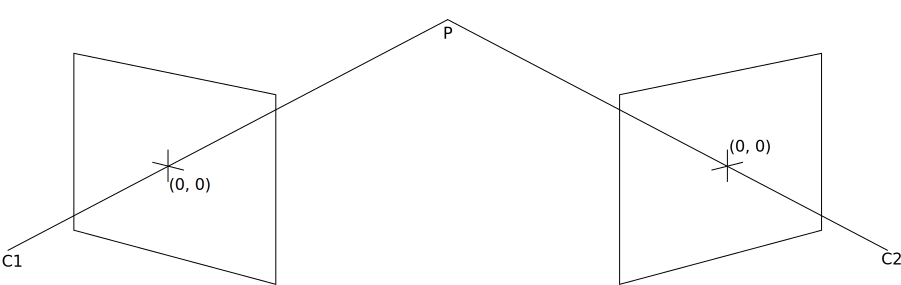
\includegraphics[width=0.75\textwidth]{images/drawing-1.pdf}
    \caption{Figure for Q1.1. $C1$ and $C2$ are the optical centers. The principal axes intersect at point $\w$ ($P$ in the figure).}
    \label{fig:theory1}
\end{figure}

\begin{your_solution}[title=Q1.1,height=6cm,width=\linewidth]
\scriptsize
Under normalized image coordinates, both the principal axes of camera C1 and C2 intersect at a 3D point {\bf w}, plus C1 intercepting at image plane at coordinate $x_1$ = $\begin{bmatrix} 0 \\ 0 \\ 1 \end{bmatrix}$ (in homogeneous coordinate) and C2 intercepting at image plane at coordinate $x_2$ = $\begin{bmatrix} 0 \\ 0 \\ 1 \end{bmatrix}$ (in homogeneous coordinate), then $x_1$ and $x_2$ satisify the following equation: $x_2^T F x_1 = 0$, where F = $\begin{bmatrix}
	F_{11} & F_{12} & F_{13} \\
	F_{21} & F_{22} & F_{23} \\
	F_{31} & F_{32} & F_{33}
\end{bmatrix}$.
When we plug in $x_1$ and $x_2$, it shows that $\begin{bmatrix} 0 & 0 & 1 \end{bmatrix}
\begin{bmatrix}
F_{11} & F_{12} & F_{13} \\
F_{21} & F_{22} & F_{23} \\
F_{31} & F_{32} & F_{33}
\end{bmatrix}
\begin{bmatrix} 0 \\ 0 \\ 1 \end{bmatrix} = 0$, and it results in F33 = 0.
\end{your_solution}

\subparagraph*{Q1.2}\points{5}
Consider the case of two cameras viewing an object such that the second camera differs from the first by a \emph{pure translation} that is parallel to the $x$-axis. Show that the epipolar lines in the two cameras are also parallel. Back up your argument with relevant equations. You may assume both cameras have the same intrinsics.

\begin{your_solution}[title=Q1.2,height=6cm,width=\linewidth]
\scriptsize
Since the two cameras only differ by a pure translation, the rotation matrix R = I (Identity matrix), and the translation matrix $T = [T_x, 0, 0]^T$. Then we have the following equation: $\begin{bmatrix} x_2 & y_2 & 1 \end{bmatrix} K^{-\top} E K^{-1} \begin{bmatrix} x_1 \\ y_1 \\ 1 \end{bmatrix}=0$, where E = $\begin{bmatrix} 0 & 0 & 0 \\ 0 & 0 & -T_x \\ 0 & T_x & 0 \end{bmatrix}$. We can view $K^{-1} \begin{bmatrix} x \\ y \\ 1 \end{bmatrix} = \begin{bmatrix} x_n \\ y_n \\ 1 \end{bmatrix}$ in normalized camer coordinates, then the above equation would be $\begin{bmatrix} x_{n2} & y_{n2} & 1 \end{bmatrix} E \begin{bmatrix} x_{n1} \\ y_{n1} \\ 1 \end{bmatrix}=0$. We now have epipolar line in C2 as $l_2$ = $E \begin{bmatrix} x_{n1} \\ y_{n1} \\ 1 \end{bmatrix} = \begin{bmatrix} 0 \\ -T_x \\ T_xy_{n1} \end{bmatrix}$ $\rightarrow$ $x_{n2}^T\begin{bmatrix} 0 \\ -T_x \\ T_xy_{n1} \end{bmatrix} = -y_{n2}T_x + T_xy_{n1} = 0$ , and epipolar line in C1 as $l_1$ = $E^T \begin{bmatrix} x_{n2} \\ y_{n2} \\ 1 \end{bmatrix} = \begin{bmatrix} 0 \\ T_x \\ -T_xy_{n2} \end{bmatrix}$ $\rightarrow$ $x_{n1}^T\begin{bmatrix} 0 \\ T_x \\ -T_xy_{n2} \end{bmatrix}$ = $y_{n1}T_x - T_xy_{n2} = 0$. We can see that $l_1$ and $l_2$  are both horizontal lines (parallel to the x-axis), and they are parallel to each other.


%We can view $\begin{bmatrix} x_2 & y_2 & 1\end{bmatrix} K^{-\top}$ as camera coordinate of $C2 = [C_{2x}, C_{2y}, C_{2z}]$, and $K^{-1} \begin{bmatrix} x_1 \\ y_1 \\ 1 \end{bmatrix}$ as camera coordinate of $C1 = [C_{1x}, C_{1y}, C_{1z}]^T$. Then, we have the following equation: $\begin{bmatrix} C_{2x} & C_{2y} & C_{2z} \end{bmatrix} E \begin{bmatrix} C_{1x} \\ C_{1y} \\ C_{1z} \end{bmatrix}=0$. The epopolar line in camera C2 = K E  $\begin{bmatrix} C_{1x} \\ C_{1y} \\ C_{1z} \end{bmatrix}$ = $K [0, -T_x C_{1z}, T_xC_{1y}]$

%It turns out to the equation: $\frac{C_{2y}}{C_{2z}} = \frac{C_{1y}}{C_{1z}}$. After multiplying both camera coordinates: $C1 = [C_{1x}, C_{1y}, C_{1z}]^T$ and $C2 = [C_{2x}, C_{2y}, C_{2z}]^T$ by the same intrinsic matrix K and applying the equation: $\frac{C_{2y}}{C_{2z}} = \frac{C_{1y}}{C_{1z}}$, we get image coordinates $y_2$ = $y_1$, showing that the epipolar lines in the two cameras are parallel.
\end{your_solution}

\subparagraph*{Q1.3}\points{5}
Suppose we have an inertial sensor that gives us the accurate positions ($\R_i$ and $\t_i$, the rotation matrix and translation vector) of the robot at time $i$. What will be the effective rotation ($\R_{rel}$) and translation ($\t_{rel}$) between two frames at different time stamps? Suppose the camera intrinsics ($\K$) are known, express the essential matrix ($\E$) and the fundamental matrix ($\F$) in terms of $\K$, $\R_{rel}$ and $\t_{rel}$.

\begin{figure}[h]
    \centering
    \includegraphics[width=0.75\textwidth]{images/F_E}
    \caption{Figure for Q1.3. $C1$ and $C2$ are the optical centers. The rotation and the translation is obtained using inertial sensors. $\R_{rel}$ and $\t_{rel}$ are the relative rotation and translation between two frames.}
    \label{fig:theory3}
\end{figure}

\begin{your_solution}[title=Q1.3,height=17cm,width=\linewidth]
Assume P = $\begin{bmatrix} X_P \\ Y_P \\ Z_P \end{bmatrix}$ is the 3D interception point of camera at time 1 and time 2, that is, camera C1 and C2. Then we have image point in C1 and C2 as $x_1$ and $x_2$ as the following equations:
\begin{align}
	\lambda_1 \begin{bmatrix} x_1 \\ y_1 \\ 1 \end{bmatrix} = K(R_1 \begin{bmatrix} X_P \\ Y_P \\ Z_P \end{bmatrix}) + t_1 \\
	\lambda_2 \begin{bmatrix} x_2 \\ y_2 \\ 1 \end{bmatrix} = K(R_2 \begin{bmatrix} X_P \\ Y_P \\ Z_P \end{bmatrix}) + t_2
\end{align}
The $\lambda_1$ and $\lambda_2$ are the scalar for homogeneous coordinates. When we substitute $\begin{bmatrix} X_P \\ Y_P \\ Z_P \end{bmatrix}$ with $\begin{bmatrix} x_1 \\ y_1 \\ 1 \end{bmatrix}$ in equation (2), then we have the following equation:
\begin{equation}
\begin{split}
	\lambda_2 \begin{bmatrix} x_2 \\ y_2 \\ 1 \end{bmatrix} &= K(R_2 R_1^{-1} (K^{-1} \lambda_1 \begin{bmatrix} x_1 \\ y_1 \\ 1 \end{bmatrix} - t_1) + t_2) \\
	 &= K R_2 R_1^{-1} K^{-1} \lambda_1 \begin{bmatrix} x_1 \\ y_1 \\ 1 \end{bmatrix} - K R_2 R_1^{-1} t_1 + K t_2 \\
	 &= K R_{rel} K^{-1} \lambda_1 \begin{bmatrix} x_1 \\ y_1 \\ 1 \end{bmatrix} + K t_{rel}
\end{split}
\end{equation}
Accordingly, $R_{rel}$ = $R_2 R_1^{-1}$, and $t_{rel} = t_2 - R_2 R_1^{-1} t_1$. Also, the essential matrix E is the cross product of $t_{rel}$ and $R_{rel}$: $E = t_{rel} \times R_{rel}$, and the fundamental matrix F is: $F = K^{-T}(t_{rel} \times R_{rel}) K^{-1}$.


\end{your_solution}
\newpage

\part{Practice}
\label{part:practice}

\section{Overview}

In this part you will begin by implementing the 8-point algorithm seen in class to estimate the fundamental matrix from corresponding points in two images (\autoref{sec:fundmatrix}).  Next, given the fundamental matrix and calibrated intrinsics (which will be provided) you will compute the essential matrix and use this to compute a 3D metric reconstruction from 2D correspondences using triangulation (\autoref{sec:essmatrix}). Then, you will implement a method to automatically match points taking advantage of epipolar constraints and make a 3D visualization of the results (\autoref{sec:viz}). Finally, you will implement RANSAC and bundle adjustment to further improve your algorithm (\autoref{sec:bundle}).
\section{Fundamental Matrix Estimation}
\label{sec:fundmatrix}

In this section you will explore different methods of estimating the fundamental matrix given a pair of images. In the $\texttt{data/}$ directory, you will find two images (see \autoref{fig:temple_dataset}) from the Middlebury multi-view dataset\footnote{\url{http://vision.middlebury.edu/mview/data/}}, which is used to evaluate the performance of modern 3D reconstruction algorithms.
\begin{figure}[h]
    \centering
    \includegraphics[width=0.35\textwidth]{images/im1.png}\ \
    \includegraphics[width=0.35\textwidth]{images/im2.png}
\caption{\texttt{Temple} images for this assignment}
    \label{fig:temple_dataset}
\end{figure}


\subsection{The Eight Point Algorithm}

The 8-point algorithm (discussed in class, and outlined in Section 8.1 of \cite{forsyth2002computer}) is arguably the simplest method for estimating the fundamental matrix. For this section, you can use provided correspondences you can find in \texttt{data/some\_corresp.npz}.


\subparagraph*{Q2.1}\points{10}
\begin{figure}[t]
    \centering
    \includegraphics[width=0.8\textwidth]{images/q1_3_epi.png}
    \caption{\texttt{displayEpipolarF} in \texttt{helper.py} creates a GUI for visualizing epipolar lines}
    \label{fig:epigui}
\end{figure}
Finish the function \texttt{eightpoint} in \texttt{q2\_1\_eightpoint.py}. Make sure you follow the signature for this portion of the assignment:
\begin{center}
    \texttt{F = eightpoint(pts1, pts2, M)}
\end{center}
where \texttt{pts1} and \texttt{pts2} are $N \times 2$ matrices corresponding to the $(x,y)$ coordinates of the $N$ points in the first and second image respectively. \texttt{M} is a scale parameter.
\begin{itemize}
    \item You should scale the data as was discussed in class, by dividing each coordinate by $M$ (the maximum of the image's width and height). After computing $\F$, you will have to ``unscale'' the fundamental matrix.
    \\\emph{Hint:} If $\x_{normalized} = \T\x$, then $\F_{unnormalized} = \T^T \F \T$.
    \\You must enforce the singularity condition of $\F$ before unscaling.

    \item You may find it helpful to refine the solution by using local minimization.  This probably won't fix a completely broken solution, but may make a good solution better by locally minimizing a geometric cost function. For this we have provided a helper function \texttt{refineF} in \texttt{helper.py} taking in $\F$ and the two sets of points, which you can call from \texttt{eightpoint} before unscaling \texttt{F}.

    \item Remember that the $x$-coordinate of a point in the image is its column entry, and $y$-coordinate is the row entry. Also note that eight-point is just a figurative name, it just means that you need at least 8 points; your algorithm should use an over-determined system ($N>8$ points).

    \item To visualize the correctness of your estimated $\F$, use the function \texttt{displayEpipolarF} in \texttt{helper.py}, which takes in $\F$, and the two images. This GUI lets you select a point in one of
    the images and visualize the corresponding epipolar line in the other image (\autoref{fig:epigui}).
    
    \item In addition to visualization, we also provide a test code snippet in \texttt{q2\_1\_eightpoint.py} which uses helper function \texttt{calc\_epi\_error} to evaluate the quality of the estimated fundamental matrix. This function calculates the distance between the estimated epipolar line and the corresponding points. For the eight point algorithm, the error should on average be $< 1$. 

\end{itemize}

\deliver{
\textbf{Output:} Save your matrix $\F$ and scale \texttt{M} to the file \texttt{q2\_1.npz}.\\
\textbf{In your write-up:} 
\begin{itemize}
    \item Write your recovered $\F$
    \item Include an image of some example output of \texttt{displayEpipolarF}
    \item Include the code snippet of \texttt{eightpoint} function
\end{itemize}
}

\begin{your_solution}[title=Q2.1,height=23.2cm,width=\linewidth]
As in the output: $./q2\_1.npz$, the recovered F is: 
\newline

$\begin{pmatrix}
	-2.19293792e^{-07} &  2.95926413e^{-05} & -2.51886251e^{-01} \\
	1.28064423e^{-05}  & -6.64493522e^{-07} &  2.63771761e^{-03} \\
	2.42228993e^{-01}  & -6.82585388e^{-03} &  1.00000000e^{+00}
\end{pmatrix}$
\newline

Besides, M = 640.
\newline
The following \autoref{fig:Q2_1_result} shows the result of the Eight Point Algorithm:
\newline
\begin{minipage}{1\linewidth}
	\centering
	\includegraphics[width=1\linewidth, height=0.39\columnwidth]{../Q2_1_result.png}
	\refstepcounter{figure}  % Increment the figure counter
	\textbf{Figure \ref{fig:Q2_1_result}:} Result of the Eight Point Algorithm  % Manually add a caption/title
	\label{fig:Q2_1_result}         % Label for referencing	
\end{minipage}
\newline

The following \autoref{fig:first_image} and \autoref{fig:second_image} show the code snippet of the Eight Point Algorithm in q2\_1\_eightpoint.py:
\newline
\begin{minipage}{0.48\linewidth}
	\centering
	\includegraphics[width=\linewidth]{../Q2_1_cns1.png}
	\refstepcounter{figure}  % Increment the figure counter
    \textbf{Figure \ref{fig:first_image}:} First Code Snippet  % Manually add a caption/title
	\label{fig:first_image}         % Label for referencing	
\end{minipage}
\hfill
\begin{minipage}{0.48\linewidth}
	\centering
	\includegraphics[width=\linewidth, height=1.43\columnwidth]{../Q2_1_cns2.png}
	\refstepcounter{figure}  % Increment the figure counter
	\textbf{Figure \ref{fig:second_image}:} Second Code Snippet  % Manually add a caption/title
	\label{fig:second_image}         % Label for referencing
\end{minipage}


\end{your_solution}

\subsection{The Seven Point Algorithm (Extra Credit)}
% The Seven-Point Algorithm

Since the fundamental matrix only has seven degrees of freedom, it is possible to calculate $\textbf{F}$ using only seven-point correspondences. This requires solving a polynomial equation.  In this section, you will implement the seven-point algorithm  (outlined in this \href{https://imkaywu.github.io/blog/2017/06/fundamental-matrix/}{\textcolor{blue}{post}}). 

\subparagraph*{Q2.2} \points{Extra Credit - 15}
Finish the function \texttt{sevenpoint} in \texttt{q2\_2\_sevenpoint.py}. Make sure you follow the signature for this portion of the assignment:
\begin{center}
    \texttt{Farray = sevenpoint(pts1, pts2, M)}
\end{center}
where pts1 and pts2 are $7 \times 2$ matrices containing the correspondences and \texttt{M} is the normalizer (use the maximum of the image's height and width), and \texttt{Farray} is a list array of length either 1 or 3 containing Fundamental matrix/matrices. Use \texttt{M} to normalize the point values between $[0,1]$ and remember to ``unnormalize" your computed $\textbf{F}$ afterward.

Manually select $7$ points from the provided point in \texttt{data/some\_corresp.npz}, and use these points to recover a fundamental matrix $\textbf{F}$. Use \texttt{calc\_epi\_error} in \texttt{helper.py} to calculate the error to pick the best one, and use \texttt{displayEpipolarF} to visualize and verify the solution.

\deliver{
\textbf{Output:} Save your matrix $\F$ and scale \texttt{M} to the file \texttt{q2\_2.npz}.\\
\textbf{In your write-up: }
\begin{itemize}
    \item Write your recovered $\textbf{F}$ 
    \item Include an image of some example output of \texttt{displayEpipolarF}
    \item Include the code snippet of \texttt{sevenpoint} function
\end{itemize}
}

\begin{your_solution}[title=Q2.2,height=21.5cm,width=\linewidth]
As in the output: $./q2\_2.npz$, the recovered F is: 
\newline

$\begin{pmatrix}
8.10457547e^{-07} &  8.90918216e^{-06} & -2.01028479e^{-01} \\
2.63329923e^{-05} & -6.00542314e^{-07} &  6.97427247e^{-04} \\
1.92182103e^{-01} & -4.20123320e^{-03} &  1.00000000e^{+00}
\end{pmatrix}$
\newline

Besides, M = 640.
\newline
The following \autoref{fig:Q2_2_result} shows the result of the Eight Point Algorithm:
\newline
\begin{minipage}{1\linewidth}
	\centering
	\includegraphics[width=\linewidth]{../Q2_2_result.png}
	\refstepcounter{figure}  % Increment the figure counter
	\textbf{Figure \ref{fig:Q2_2_result}:} Result of the Seven Point Algorithm  % Manually add a caption/title
	\label{fig:Q2_2_result}         % Label for referencing	
\end{minipage}
\newline

The following \autoref{fig:Q2_2_cns1}, \autoref{fig:Q2_2_cns2}, \autoref{fig:Q2_2_cns3} and \autoref{fig:Q2_2_cns4} show the code snippet of the Seven Point Algorithm in q2\_2\_sevenpoint.py:
\newline


\begin{minipage}{0.48\linewidth}
	\centering
	\includegraphics[width=\linewidth]{../Q2_2_cns1.png}
	\refstepcounter{figure}  % Increment the figure counter
	\textbf{Figure \ref{fig:Q2_2_cns1}:} First Code Snippet  % Manually add a caption/title
	\label{fig:Q2_2_cns1}         % Label for referencing	
\end{minipage}
\hfill
\begin{minipage}{0.48\linewidth}
	\centering
	\includegraphics[width=\linewidth]{../Q2_2_cns2.png}
	\refstepcounter{figure}  % Increment the figure counter
	\textbf{Figure \ref{fig:Q2_2_cns2}:} Second Code Snippet  % Manually add a caption/title
	\label{fig:Q2_2_cns2}         % Label for referencing
\end{minipage}	
\newline
\end{your_solution}
\newpage
\begin{your_solution}[title=Q2.2 continued,height=10.0cm,width=\linewidth]
\begin{minipage}{0.48\linewidth}
	\centering
	\includegraphics[width=\linewidth]{../Q2_2_cns3.png}
	\refstepcounter{figure}  % Increment the figure counter
	\textbf{Figure \ref{fig:Q2_2_cns3}:} Third Code Snippet  % Manually add a caption/title
	\label{fig:Q2_2_cns3}         % Label for referencing	
\end{minipage}
\hfill
\begin{minipage}{0.48\linewidth}
	\centering
	\includegraphics[width=\linewidth]{../Q2_2_cns4.png}
	\refstepcounter{figure}  % Increment the figure counter
	\textbf{Figure \ref{fig:Q2_2_cns4}:} Fourth Code Snippet  % Manually add a caption/title
	\label{fig:Q2_2_cns4}         % Label for referencing
\end{minipage}
\end{your_solution}

\newpage
\section{Metric Reconstruction}
\label{sec:essmatrix}

You will compute the camera matrices and triangulate the 2D points to obtain the 3D scene structure. To obtain the Euclidean scene structure, first convert the fundamental matrix $\F$ to an essential matrix $\E$. Examine the lecture notes and the textbook to find out how to do this when the internal camera calibration matrices $\K_1$ and $\K_2$ are known; these are provided in \texttt{data/intrinsics.npz}.

\subparagraph*{Q3.1}\points{5}
Complete the function \texttt{essentialMatrix} in \texttt{q3\_1\_essential\_matrix.py} to compute the essential matrix $\E$ given $\F$, $\K_1$ and $\K_2$ with the signature:
\begin{center}
    \texttt{E = essentialMatrix(F, K1, K2)}
\end{center}

\deliver{
\textbf{Output:} Save your estimated $\E$ using $\F$ from the eight-point algorithm to \texttt{q3\_1.npz}.\\
\textbf{In your write-up: }
\begin{itemize}
    \item Write your estimated $\textbf{E}$
    \item Include the code snippet of \texttt{essentialMatrix} function
\end{itemize}
}

\begin{your_solution}[title=Q3.1,height=12.5cm,width=\linewidth]
	As in the output: $./q3\_1.npz$, the recovered E is: 
	\newline
	
	$\begin{pmatrix}
	-5.06923074e^{-01} &  6.86542875e^{+01} & -3.71961318e^{+02}\\
	2.97106690e^{+01}  & -1.54718732e^{+00} &  9.68232032e^{+00}\\
	3.72990948e^{+02}  &  2.98549953e^{+00} &  1.50354471e^{-01}
	\end{pmatrix}$
	\newline
	
The following \autoref{fig:Q3_1_cns} shows the code snippet of the q3\_1\_essential\_matrix.py:
\newline

%\begin{minipage}{1\linewidth}
	%\centering
	%\includegraphics[width=0.5\linewidth]{../Q3_1_cns.png}
	%\refstepcounter{figure}  % Increment the figure counter
	%\textbf{Figure \ref{fig:Q3_1_cns}:} Code Snippet  % Manually add a caption/title
	%\label{fig:Q3_1_cns}         % Label for referencing	
%\end{minipage}	

\begin{minipage}{1\linewidth}
	\centering
	\hspace{0.12\linewidth} 
	\includegraphics[width=0.5\linewidth]{../Q3_1_cns.png}  % Adjust the width to 50% of the line width
	\refstepcounter{figure}  % Increment the figure counter
	\newline
	\textbf{Figure \thefigure:} Code Snippet % Manually add a caption/title
	\label{fig:Q3_1_cns}  % Label for referencing
\end{minipage}

\end{your_solution}

\hfill\\

Given an essential matrix, it is possible to retrieve the projective camera matrices $\M_1$ and $\M_2$ from it.  Assuming $\M_1$ is fixed at $[\I,0]$, $\M_2$ can be retrieved up to a scale and four-fold rotation ambiguity. For details on recovering $\M_2$, see section 11.3 in Szeliski. We have provided you with the function \texttt{camera2} in \texttt{python/helper.py} to recover the four possible $\M_2$ matrices given $\E$.

\textbf{Note: } The matrices $\M1$ and $\M2$ here are of the form: 
$\M_1 = \begin{bmatrix}\I | 0\end{bmatrix} $ and $\M_2 = \begin{bmatrix}\R | \t\end{bmatrix} $.

\subparagraph*{Q3.2}\points{10}
Using the above, complete the function \texttt{triangulate} in \texttt{q3\_2\_triangulate.py} to triangulate a set of 2D coordinates in the image to a set of 3D points with the signature:
\begin{center}
    \texttt{[w, err] = triangulate(C1, pts1, C2, pts2)}
\end{center}
where \texttt{pts1} and \texttt{pts2} are the $N \times 2$ matrices with the 2D image coordinates and \texttt{w} is an $N \times 3$ matrix with the corresponding 3D points per row.  \texttt{C1} and \texttt{C2} are the $3 \times 4$ camera matrices. Remember that you will need to multiply the given intrinsics matrices with your solution for the canonical camera matrices to obtain the final camera matrices. Various methods exist for triangulation -
probably the most familiar for you is based on least squares (see \cite{szeliski2022computer} Chapter 7 if you want to learn about other methods).

For each point $i$, we want to solve for 3D coordinates $\w_i = \begin{bmatrix}x_i, y_i, z_i\end{bmatrix}^T$, such that when they are projected back to the two images, they are close to the original 2D points. To project the 3D coordinates back to 2D images, we first write $\w_i$ in homogeneous coordinates, and compute $\mathbf{C}_1 \tilde{\w_i}$ and $\mathbf{C}_2 \tilde{\w_i}$ to obtain the 2D homogeneous coordinates projected to camera $1$ and camera $2$, respectively.

For each point $i$, we can write this problem in the following form:
\begin{align*}
\mathbf{A}_i\w_i = 0,
\end{align*}
where $\mathbf{A}_i$ is a $4\times 4$ matrix, and $\tilde{\w_i}$ is a $4\times 1$ vector of the 3D coordinates in the homogeneous form. Then, you can obtain the homogeneous least-squares solution (discussed in class) to solve for each $\w_i$.

Once you have implemented triangulation, check the performance by looking at the reprojection error:  
\begin{align*}
\texttt{err} = \sum_i \|\x_{1i}, \widehat{\x_{1i}}\|^2 + \|\x_{2i}, \widehat{\x_{2i}}\|^2    
\end{align*}
where $\widehat{\x_{1i}} = Proj(\mathbf{C}_1, \w_i)$ and $\widehat{\x_{2i}} = Proj(\mathbf{C}_2, \w_i)$. You should see an error less than 500. Ours is around 350. 

\textbf{Note: } \texttt{C1} and \texttt{C2} here are projection matrices of the form:
$\mathbf{C}_1 = \mathbf{K}_1\mathbf{M}_1 = \mathbf{K}_1 \begin{bmatrix}
\I | 0
\end{bmatrix} $ and $\mathbf{C}_2 =  \mathbf{K}_2\mathbf{M}_2 = \mathbf{K}_2 \begin{bmatrix}
\R | \t
\end{bmatrix}$.

\deliver{
\textbf{In your write-up:} 
\begin{itemize}
    \item Write down the expression for the matrix $\mathbf{A}_i$ for triangulating a pair of 2D coordinates in the image to a 3D point.
    \item Include the code snippet of \texttt{triangulate} function.
\end{itemize}
}

\begin{your_solution}[title=Q3.2,height=22.5cm,width=\linewidth]
Assume that $\mathbf{w}_i = \begin{bmatrix} x_i \\ y_i \\ z_i \end{bmatrix}$ is the 3D coordinates at point i, and $\tilde{\mathbf{w}}_i = \begin{bmatrix} x_i \\ y_i \\ z_i \\ 1 \end{bmatrix}$ is its homogeneous coordinate. Besides, $u_1 = \lambda_1\begin{bmatrix} u_{xi_{1}} \\ u_{yi_{1}} \\ 1 \end{bmatrix}$ is the 2D projected homogeneous coordinates on camera1 and $u_2 = \lambda_2\begin{bmatrix} u_{xi_{2}} \\ u_{yi_{2}} \\ 1 \end{bmatrix}$ is the 2D projected homogeneous coordinates on camera2. Let us define the C1 and C2 camera matrix as the following:
\begin{align}
	C1 = \begin{bmatrix}
		c_{1_{11}} & c_{1_{12}} & c_{1_{13}} & c_{1_{14}} \\
		c_{1_{21}} & c_{1_{22}} & c_{1_{23}} & c_{1_{24}} \\
		c_{1_{31}} & c_{1_{32}} & c_{1_{33}} & c_{1_{34}}
	\end{bmatrix} \\
	C2 = \begin{bmatrix}
	c_{2_{11}} & c_{2_{12}} & c_{2_{13}} & c_{2_{14}} \\
	c_{2_{21}} & c_{2_{22}} & c_{2_{23}} & c_{2_{24}} \\
	c_{2_{31}} & c_{2_{32}} & c_{2_{33}} & c_{2_{34}}
	\end{bmatrix}
	%\lambda_1 \begin{bmatrix} x_1 \\ y_1 \\ 1 \end{bmatrix} = K(R_1 \begin{bmatrix} X_P \\ Y_P \\ Z_P \end{bmatrix}) + t_1 \\
	%\lambda_2 \begin{bmatrix} x_2 \\ y_2 \\ 1 \end{bmatrix} = K(R_2 \begin{bmatrix} X_P \\ Y_P \\ Z_P \end{bmatrix}) + t_2
\end{align}
Then, we have the following two equations:
\begin{align}
	 \lambda_1\begin{bmatrix} u_{xi_{1}} \\ u_{yi_{1}} \\ 1 \end{bmatrix} = \begin{bmatrix}
		c_{1_{11}} & c_{1_{12}} & c_{1_{13}} & c_{1_{14}} \\
		c_{1_{21}} & c_{1_{22}} & c_{1_{23}} & c_{1_{24}} \\
		c_{1_{31}} & c_{1_{32}} & c_{1_{33}} & c_{1_{34}}
	\end{bmatrix} \begin{bmatrix} x_i \\ y_i \\ z_i \\ 1 \end{bmatrix} \\
	 \lambda_2\begin{bmatrix} u_{xi_{2}} \\ u_{yi_{2}} \\ 1 \end{bmatrix} = \begin{bmatrix}
		c_{2_{11}} & c_{2_{12}} & c_{2_{13}} & c_{2_{14}} \\
		c_{2_{21}} & c_{2_{22}} & c_{2_{23}} & c_{2_{24}} \\
		c_{2_{31}} & c_{2_{32}} & c_{2_{33}} & c_{2_{34}}
	\end{bmatrix} \begin{bmatrix} x_i \\ y_i \\ z_i \\ 1 \end{bmatrix}
\end{align}
After multiplying both equation (6) and (7) out, dividing x and y coordinates by the z coordinate, and rearranging the equations, we get the following equation:
\begin{align}
	\begin{bmatrix}
		c_{1_{11}}-u_{xi_{1}}c_{1_{31}} & c_{1_{12}}-u_{xi_{1}}c_{1_{32}} & c_{1_{13}}-u_{xi_{1}}c_{1_{33}} & c_{1_{14}}-u_{xi_{1}}c_{1_{34}} \\
		c_{1_{21}}-u_{yi_{1}}c_{1_{31}} & c_{1_{22}}-u_{yi_{1}}c_{1_{32}} & c_{1_{23}}-u_{yi_{1}}c_{1_{33}} & c_{1_{24}}-u_{yi_{1}}c_{1_{34}} \\
		c_{2_{11}}-u_{xi_{2}}c_{2_{31}} & c_{2_{12}}-u_{xi_{2}}c_{2_{32}} & c_{2_{13}}-u_{xi_{2}}c_{2_{33}} & c_{2_{14}}-u_{xi_{2}}c_{2_{34}} \\
		c_{2_{21}}-u_{yi_{2}}c_{2_{31}} & c_{2_{22}}-u_{yi_{2}}c_{2_{32}} & c_{2_{23}}-u_{yi_{2}}c_{2_{33}} & c_{2_{24}}-u_{yi_{2}}c_{2_{34}}
	\end{bmatrix} \begin{bmatrix} x_i \\ y_i \\ z_i \\ 1 \end{bmatrix} = 0
\end{align}
Accordingly, we have A matrix: \newline
\begin{align}
A = \begin{bmatrix}
	c_{1_{11}}-u_{xi_{1}}c_{1_{31}} & c_{1_{12}}-u_{xi_{1}}c_{1_{32}} & c_{1_{13}}-u_{xi_{1}}c_{1_{33}} & c_{1_{14}}-u_{xi_{1}}c_{1_{34}} \\
	c_{1_{21}}-u_{yi_{1}}c_{1_{31}} & c_{1_{22}}-u_{yi_{1}}c_{1_{32}} & c_{1_{23}}-u_{yi_{1}}c_{1_{33}} & c_{1_{24}}-u_{yi_{1}}c_{1_{34}} \\
	c_{2_{11}}-u_{xi_{2}}c_{2_{31}} & c_{2_{12}}-u_{xi_{2}}c_{2_{32}} & c_{2_{13}}-u_{xi_{2}}c_{2_{33}} & c_{2_{14}}-u_{xi_{2}}c_{2_{34}} \\
	c_{2_{21}}-u_{yi_{2}}c_{2_{31}} & c_{2_{22}}-u_{yi_{2}}c_{2_{32}} & c_{2_{23}}-u_{yi_{2}}c_{2_{33}} & c_{2_{24}}-u_{yi_{2}}c_{2_{34}}
\end{bmatrix}
\end{align}
\end{your_solution}

\begin{your_solution}[title=Q3.2 continued,height=15.5cm,width=\linewidth]
The following \autoref{fig:Q3_2_cns} shows the code snippet of triangulate() in the q3\_2triangulate.py:
\newline

\begin{minipage}{1\linewidth}
	\centering
	\hspace{0.12\linewidth} 
	\includegraphics[width=0.7\linewidth]{../Q3_2_cns.png}  % Adjust the width to 50% of the line width
	\refstepcounter{figure}  % Increment the figure counter
	\newline
	\textbf{Figure \thefigure:} Code Snippet % Manually add a caption/title
	\label{fig:Q3_2_cns}  % Label for referencing
\end{minipage}
\end{your_solution}

\subparagraph*{Q3.3}\points{10}
Complete the function \texttt{findM2} in \texttt{q3\_2\_triangulate.py} to obtain the correct \texttt{M2} from \texttt{M2s} by testing the four solutions through triangulations.\\Use the correspondences from \texttt{data/some\_corresp.npz}.

\deliver{
\textbf{Output:} Save the correct \texttt{M2},
the corresponding \texttt{C2}, and 3D points \texttt{P} to \texttt{q3\_3.npz}.\\ 
\textbf{In your writeup:} Include the code snippet of \texttt{findM2} function.
}

\begin{your_solution}[title=Q3.3,height=14.5cm,width=\linewidth]
	The following \autoref{fig:Q3_3_cns} shows the code snippet of findM2() in the q3\_2triangulate.py:
	\newline
	
	\begin{minipage}{1\linewidth}
		\centering
		\hspace{0.12\linewidth} 
		\includegraphics[width=0.7\linewidth]{../Q3_3_cns.png}  % Adjust the width to 50% of the line width
		\refstepcounter{figure}  % Increment the figure counter
		\newline
		\textbf{Figure \thefigure:} Code Snippet % Manually add a caption/title
		\label{fig:Q3_3_cns}  % Label for referencing
	\end{minipage}
\end{your_solution}


\newpage

\section{3D Visualization}
\label{sec:viz}
You will now create a 3D visualization of the temple images. By treating our two images as a stereo-pair, we can triangulate corresponding points in each image, and render their 3D locations.

\subparagraph*{Q4.1}\points{15} In \texttt{q4\_1\_epipolar\_correspondence.py} finish the function \\ \texttt{epipolarCorrespondence} with the signature:
\begin{center}
    \texttt{[x2, y2] = epipolarCorrespondence(im1, im2, F, x1, y1)}
\end{center}
This function takes in the $x$ and $y$ coordinates of a pixel on \verb!im1! and your fundamental matrix $\F$, and returns the coordinates of the pixel on \verb!im2! which correspond to the input point. The match is obtained by computing the similarity of a small window around the $(x_1, y_1)$ coordinates in \verb!im1! to various windows around possible matches in the \verb!im2! and returning the closest.

Instead of searching for the matching point at every possible location in \verb!im2!, we can use $\F$ and simply search over the set of pixels that lie along the epipolar line (recall that the epipolar line passes through a single point in \verb!im2!  which corresponds to the point $(x_1, y_1)$ in \verb!im1!).

There are various possible ways to compute the window similarity. For this assignment, simple methods such as the Euclidean or Manhattan distances between the intensity of the pixels should suffice.  See \cite{szeliski2022computer} chapter 11, on stereo matching, for a brief overview of these and other methods.

\textbf{\emph{Implementation hints:}}
\begin{itemize}
    \item Experiment with various window sizes.
    \item It may help to use a Gaussian weighting of the window, so that the center has greater influence than the periphery.
    \item Since the two images only differ by a small amount, it might be beneficial to consider matches for which the distance from $(x_1, y_1)$ to $(x_2, y_2)$ is small.
\end{itemize}
To help you test your \texttt{epipolarCorrespondence}, we have included a helper function \texttt{epipolarMatchGUI} in \texttt{q4\_1\_epipolar\_correspondence.py}, which takes in two images and the fundamental matrix. This GUI allows you to click on a point in \texttt{im1}, and will use your function to display the corresponding point in \texttt{im2}. See \autoref{fig:epigui2}.
\begin{figure}[h]
    \centering
    \fbox{\includegraphics[width=0.8\textwidth]{images/q3gui_disp_arun.png}}
    \caption{\texttt{epipolarMatchGUI} shows the corresponding point found by
    calling \texttt{epipolarCorrespondence}}
    \label{fig:epigui2}
\end{figure}

It's not necessary for your matcher to get \textit{every} possible point right, but it should get easy points (such as those with distinctive, corner-like windows). It should also be good enough to render an intelligible representation in the next question.

\deliver{
\textbf{Output:} Save the matrix $\F$, points \texttt{pts1} and \texttt{pts2} which you used to generate the screenshot to the file \texttt{q4\_1.npz}. 

\textbf{In your write-up:} 
\begin{itemize}
    \item Include a screenshot of \texttt{epipolarMatchGUI} with some detected correspondences.
    \item Include the code snippet of \texttt{epipolarCorrespondence} function.
\end{itemize}
}

\begin{your_solution}[title=Q4.1,height=9cm,width=\linewidth]
The following \autoref{fig:Q4_1_result} shows the screenshot of epipolarMatchGUI() with some detected correspondences using the epipolarCorrespondence() function:
\newline
\begin{minipage}{1\linewidth}
	\centering
	\includegraphics[width=1\linewidth, height=0.39\columnwidth]{../Q4_1_result.png}
	\refstepcounter{figure}  % Increment the figure counter
	\textbf{Figure \ref{fig:Q4_1_result}:} Result of the epipolarCorrespondence() Function  % Manually add a caption/title
	\label{fig:Q4_1_result}         % Label for referencing	
\end{minipage}
\end{your_solution}
\newpage
\begin{your_solution}[title=Q4.1 continued,height=21.5cm,width=\linewidth]
	The following \autoref{fig:Q4_1_cns} shows the code snippet of the epipolarCorrespondence() function in q4\_1\_epipolar\_correspondence.py:	
	\newline
	
	
	\begin{minipage}{1\linewidth}
		\centering
		\includegraphics[width=1\linewidth, height=1.2\columnwidth]{../Q4_1_cns.png}
		\refstepcounter{figure}  % Increment the figure counter
		\textbf{Figure \ref{fig:Q4_1_cns}:} Code Snippet of the epipolarCorrespondence() Function  % Manually add a caption/title
		\label{fig:Q4_1_cns}         % Label for referencing	
	\end{minipage}
\end{your_solution}

\subparagraph*{Q4.2}\points{10}
Included in this homework  is a file \texttt{data/templeCoords.npz} which contains 288 hand-selected points from \verb!im1! saved in the variables \verb!x1! and \verb!y1!.

Now, we can determine the 3D location of these point correspondences using the \texttt{triangulate} function. These 3D point locations can then be plotted using the Matplotlib or plotly package. Complete the \texttt{compute3D\_pts} function in \texttt{q4\_2\_visualize.py}, which loads the necessary files from \texttt{../data/} to generate the 3D reconstruction using \texttt{scatter} function matplotlib. An example is shown in \autoref{fig:q3}. 
\begin{figure}[t]
    \centering
    \includegraphics[width=0.4\textwidth]{images/q3a.png}
    \includegraphics[width=0.4\textwidth]{images/q3b.png}\\
    \includegraphics[width=0.4\textwidth]{images/q3c.png}
    \includegraphics[width=0.4\textwidth]{images/q3d.png}
    \caption{An example point cloud}
    \label{fig:q3}
\end{figure}

\deliver{
\textbf{Output:} Again, save the matrix $\F$, matrices $\M1, \M2, \C1, \C2$ which you used to generate the screenshots to the file \texttt{q4\_2.npz}. 

\textbf{In your write-up:} 
\begin{itemize}
    \item Take a few screenshots of the 3D visualization so that the outline of the temple is clearly visible, and include them in your writeup.
    \item Include the code snippet of \texttt{compute3D\_pts} function in your write-up. 
\end{itemize}
}

\begin{your_solution}[title=Q4.2,height=17.5cm,width=\linewidth]
The following \autoref{fig:Q4_2_sh1}, \autoref{fig:Q4_2_sh2}, \autoref{fig:Q4_2_sh3} and \autoref{fig:Q4_2_sh4} show the results of the 3D visualization results of the temple:
\newline

\begin{minipage}{0.55\linewidth}
	\centering
	\includegraphics[width=\linewidth]{../Q4_2_sh1.png}
	\refstepcounter{figure}  % Increment the figure counter
	\textbf{Figure \ref{fig:Q4_2_sh1}:} First Screenshot  % Manually add a caption/title
	\label{fig:Q4_2_sh1}         % Label for referencing	
\end{minipage}
\hfill
\begin{minipage}{0.45\linewidth}
	\centering
	\includegraphics[width=\linewidth]{../Q4_2_sh2.png}
	\refstepcounter{figure}  % Increment the figure counter
	\textbf{Figure \ref{fig:Q4_2_sh2}:} Second Screenshot  % Manually add a caption/title
	\label{fig:Q4_2_sh2}         % Label for referencing
\end{minipage}	
\newline
\begin{minipage}{0.45\linewidth}
	\centering
	\includegraphics[width=\linewidth]{../Q4_2_sh3.png}
	\refstepcounter{figure}  % Increment the figure counter
	\textbf{Figure \ref{fig:Q4_2_sh3}:} Third Screenshot  % Manually add a caption/title
	\label{fig:Q4_2_sh3}         % Label for referencing	
\end{minipage}
\hfill
\begin{minipage}{0.55\linewidth}
	\centering
	\includegraphics[width=\linewidth]{../Q4_2_sh4.png}
	\refstepcounter{figure}  % Increment the figure counter
	\textbf{Figure \ref{fig:Q4_2_sh4}:} Fourth Screenshot  % Manually add a caption/title
	\label{fig:Q4_2_sh4}         % Label for referencing
\end{minipage}	
\end{your_solution}
\newpage
\begin{your_solution}[title=Q4.2 continued,height=18.5cm,width=\linewidth]
	The following \autoref{fig:Q4_2_cns} shows the code snippet of the compute3D\_pts() function in q4\_2\_visualize.py:	
	\newline
	
	
	\begin{minipage}{1\linewidth}
		\centering
		\includegraphics[width=1\linewidth, height=1\columnwidth]{../Q4_2_cns.png}
		\refstepcounter{figure}  % Increment the figure counter
		\textbf{Figure \ref{fig:Q4_2_cns}:} Code Snippet of the compute3D\_pts() Function  % Manually add a caption/title
		\label{fig:Q4_2_cns}         % Label for referencing	
	\end{minipage}
\end{your_solution}
\newpage
\section{Bundle Adjustment}
\label{sec:bundle}

Bundle Adjustment is commonly used as the last step of every feature-based 3D reconstruction algorithm. Given a set of images depicting a number of 3D points from different viewpoints, bundle adjustment is the process of simultaneously refining the 3D coordinates along with the camera parameters. It minimizes reprojection error, which is the squared sum of distances between image points and predicted points. In this section, you will implement bundle adjustment algorithm by yourself (make use of \texttt{q5\_bundle\_adjustment.py} file). Specifically,

\begin{itemize}
    \item In Q5.1, you need to implement a RANSAC algorithm to estimate the fundamental matrix $\F$ and all the inliers.
    
    \item In Q5.2, you will need to write code to parameterize Rotation matrix $\mathbf{R}$ using  \href{https://en.wikipedia.org/wiki/Rodrigues\%27\_formula}{\textcolor{blue}{Rodrigues formula}} (please check \href{https://www2.cs.duke.edu/courses/fall13/compsci527/notes/rodrigues.pdf}{\textcolor{blue}{this pdf}} for a detailed explanation), which will enable the joint optimization process for Bundle Adjustment.
    
    \item In Q5.3, you will need to first write down the objective function in \texttt{rodriguesResidual}, and do the \texttt{bundleAdjustment}.
\end{itemize}

\subparagraph*{Q5.1 RANSAC for Fundamental Matrix Recovery}\points{15}
In some real world applications, manually determining correspondences is infeasible and often there will be noisy correspondences. Fortunately, the RANSAC method seen in class can be applied to the problem of fundamental matrix estimation.

Implement the above algorithm with the signature:
\begin{center}
\texttt{[F, inliers] = ransacF(pts1, pts2, M, nIters, tol)}
\end{center}
where \texttt{M} is defined in the same way as in \autoref{sec:fundmatrix} and inliers is a boolean vector of size equivalent to the number of points. Here inliers is set to true only for the points that satisfy the threshold defined for the given fundamental matrix $\F$.

We have provided some noisy correspondences in \texttt{some\_corresp\_noisy.npz} in which around $75\%$ of the points are inliers. 

\deliver{
\textbf{In your write-up:} Compare the result of RANSAC with the result of the eightpoint when ran on the noisy correspondences. Briefly explain the error metrics you used, how you decided which points were inliers, and any other optimizations you may have made. \texttt{nIters} is the maximum number of iterations of RANSAC and \texttt{tol} is the tolerance of the error to be considered as inliers. Discuss the effect on the Fundamental matrix by varying these values. \textbf{Please include the code snippet of the \texttt{ransacF} function in your write-up.}
}

\begin{itemize}
    \item \emph{Hints:} Use the Eight or Seven point algorithm to compute the fundamental matrix from the minimal set of points. Then compute the inliers, and refine your estimate using all the inliers.
\end{itemize}

\begin{your_solution}[title=Q5.1,height=20.5cm,width=\linewidth]
The following \autoref{fig:Q5_1_ran_res} shows the screenshot of RANSAC Seven Point algorithm result:
\newline

\begin{minipage}{1\linewidth}
	\centering
	\includegraphics[width=1\linewidth, height=0.39\columnwidth]{../Q5_1_ransac_seven_result.png}
	\refstepcounter{figure}  % Increment the figure counter
	\textbf{Figure \ref{fig:Q5_1_ran_res}:} Result of the RANSAC Seven Point Algorithm  % Manually add a caption/title
	\label{fig:Q5_1_ran_res}         % Label for referencing	
\end{minipage}
\newline

The following \autoref{fig:Q5_1_eig_res} shows the screenshot of Eight Point algorithm result:
\newline

\begin{minipage}{1\linewidth}
	\centering
	\includegraphics[width=1\linewidth, height=0.39\columnwidth]{../Q5_1_eight_result.png}
	\refstepcounter{figure}  % Increment the figure counter
	\textbf{Figure \ref{fig:Q5_1_eig_res}:} Result of the Eight Point Algorithm  % Manually add a caption/title
	\label{fig:Q5_1_eig_res}         % Label for referencing	
\end{minipage}
\newline

In RANSAC Seven Point algorithm, I use nIters=1000, tol=2 to get above result, and the inlier number is 106, which is around 75\% with total number of points is 140. The reason that the RANSAC Seven Point algorithm gets better result is that the points are noisy, and it is stated in the hw3.pdf that around 75\% of these noisy points are inliers. While RANSAC Seven Point algorithm has the chance to reject outliers, the Eight Point algorithm can only use all the points, including outliers, to calculate the Fundamental Matrix, F. Accordingly, RANSAC Seven Point algorithm performs better than Eight Point algorithm under noisy data.

\end{your_solution}

\newpage
\begin{your_solution}[title=Q5.1 continued, height=22.5cm,width=\linewidth]
The following shows the results of changing the value of the 'tol' parameter.
\newline

\begin{minipage}{1\linewidth}
	\centering
	\includegraphics[width=1\linewidth, height=0.39\columnwidth]{../Q5_1_ransac_seven_tol_0.5_result.png}
	\refstepcounter{figure}  % Increment the figure counter
	\textbf{Figure \ref{fig:Q5_1_tol_0.5_res}:} Result of the RANSAC Seven Point Algorithm w/ tol=0.5, inlier rate=52.86\% % Manually add a caption/title
	\label{fig:Q5_1_tol_0.5_res}         % Label for referencing	
\end{minipage}
\hfill
\begin{minipage}{1\linewidth}
	\centering
	\includegraphics[width=1\linewidth, height=0.39\columnwidth]{../Q5_1_ransac_seven_tol_1_result.png}
	\refstepcounter{figure}  % Increment the figure counter
	\textbf{Figure \ref{fig:Q5_1_tol_1_res}:} Result of the RANSAC Seven Point Algorithm w/ tol=1, inlier rate=65.71\% % Manually add a caption/title
	\label{fig:Q5_1_tol_1_res}         % Label for referencing	
\end{minipage}
\hfill
\begin{minipage}{1\linewidth}
	\centering
	\includegraphics[width=1\linewidth, height=0.39\columnwidth]{../Q5_1_ransac_seven_tol_4_result.png}
	\refstepcounter{figure}  % Increment the figure counter
	\textbf{Figure \ref{fig:Q5_1_tol_4_res}:} Result of the RANSAC Seven Point Algorithm w/ tol=4, inlier rate=76.43\% % Manually add a caption/title
	\label{fig:Q5_1_tol_4_res}         % Label for referencing	
\end{minipage}
	
\end{your_solution}
\newpage
\begin{your_solution}[title=Q5.1 continued, height=22.5cm,width=\linewidth]
	\begin{minipage}{1\linewidth}
		\centering
		\includegraphics[width=1\linewidth, height=0.39\columnwidth]{../Q5_1_ransac_seven_tol_8_result.png}
		\refstepcounter{figure}  % Increment the figure counter
		\textbf{Figure \ref{fig:Q5_1_tol_8_res}:} Result of the RANSAC Seven Point Algorithm w/ tol=8, inlier rate=78.57\% % Manually add a caption/title
		\label{fig:Q5_1_tol_8_res}         % Label for referencing	
	\end{minipage}
	\hfill
	\begin{minipage}{1\linewidth}
		\centering
		\includegraphics[width=1\linewidth, height=0.39\columnwidth]{../Q5_1_ransac_seven_tol_16_result.png}
		\refstepcounter{figure}  % Increment the figure counter
		\textbf{Figure \ref{fig:Q5_1_tol_16_res}:} Result of the RANSAC Seven Point Algorithm w/ tol=16, inlier rate=79.29\% % Manually add a caption/title
		\label{fig:Q5_1_tol_16_res}         % Label for referencing	
	\end{minipage}
	\hfill
	\begin{minipage}{1\linewidth}
		\centering
		\includegraphics[width=1\linewidth, height=0.39\columnwidth]{../Q5_1_ransac_seven_tol_128_result.png}
		\refstepcounter{figure}  % Increment the figure counter
		\textbf{Figure \ref{fig:Q5_1_tol_128_res}:} Result of the RANSAC Seven Point Algorithm w/ tol=128, inlier rate=80\% % Manually add a caption/title
		\label{fig:Q5_1_tol_128_res}         % Label for referencing	
	\end{minipage}
\end{your_solution}
\newpage
\begin{your_solution}[title=Q5.1 continued, height=22.7cm,width=\linewidth]
As we can see from the results above that when tol is getting larger, specifically larger than 8, the result is getting worse. It is because the criteria to count a point as an inlier is getting laxer, and some of the outlier points are wrongly categorized as inliers. The resulted F is generated by some outliers and thus becomes worse. As for the necessary iteration number of RANSAC to return a good model, the value is calculated by k = $\frac{\log(1-p)}{\log(1-w^n)}$, where p = 0.999, w is about 0.75 (from hw3.pdf), and n=7, then k = 48.21, so the nIters=1000, as I set in the program for above results, should be sufficient to have RANSAC Sevent Point algorithm return a good model.
\newline

The following \autoref{fig:Q5_1_cns} shows the code snippet of the ransacF() function in q5\_bundle\_adjustment.py:	
\newline


\begin{minipage}{1\linewidth}
	\centering
	\includegraphics[width=1\linewidth, height=1\columnwidth]{../Q5_1_cns.png}
	\refstepcounter{figure}  % Increment the figure counter
	\textbf{Figure \ref{fig:Q5_1_cns}:} Code Snippet of the ransacF() Function  % Manually add a caption/title
	\label{fig:Q5_1_cns}         % Label for referencing	
\end{minipage}
\end{your_solution}

\subparagraph*{Q5.2 Rodrigues and Invsere Rodrigues}\points{15}
So far we have independently solved for camera matrix, $\mathbf{M}_j$ and 3D points $\w_i$. In bundle adjustment, we will jointly optimize the reprojection error with respect to the points $\w_i$ and the camera matrix $\C_j$.
$$
err = \sum_{ij} \|\x_{ij} - Proj(\mathbf{C}_j, \w_i)\|^2,
$$
where $\C_j = \mathbf{K}_j \mathbf{M}_j$, same as in Q3.2.

For this homework we are going to only look at optimizing the extrinsic matrix. To do this we will be parameterizing the rotation matrix $\mathbf{R}$ using Rodrigues formula to produce vector $\mathbf{r} \in \mathbb{R}^3$. Write a function that converts a Rodrigues vector $\mathbf{r}$ to a rotation matrix $\mathbf{R}$
\begin{center}
\texttt{R = rodrigues(r)}
\end{center}
as well as the inverse function that converts a rotation matrix $\mathbf{R}$ to a Rodrigues vector~$\mathbf{r}$
\begin{center}
\texttt{r = invRodrigues(R)}
\end{center}
Reference: \href{https://en.wikipedia.org/wiki/Rodrigues\%27\_formula}{\textcolor{blue}{Rodrigues formula}} and \href{https://www2.cs.duke.edu/courses/fall13/compsci527/notes/rodrigues.pdf}{\textcolor{blue}{this pdf}}.

\deliver{
\textbf{In your write-up:} Include the code snippet of \texttt{rodrigues} and \texttt{invRodrigues} functions.
}

\begin{your_solution}[title=Q5.2,height=7.5cm,width=\linewidth]
The following \autoref{fig:Q5_2_cns1}, \autoref{fig:Q5_2_cns2} show the code snippet of rodrigues() and invRodrigues() functions respectively:
\newline


\begin{minipage}{0.48\linewidth}
	\centering
	\includegraphics[width=\linewidth]{../Q5_2_cns1.png}
	\refstepcounter{figure}  % Increment the figure counter
	\textbf{Figure \ref{fig:Q5_2_cns1}:} Code Snippet of rodrigues(). % Manually add a caption/title
	\label{fig:Q5_2_cns1}         % Label for referencing	
\end{minipage}
\hfill
\begin{minipage}{0.48\linewidth}
	\centering
	\includegraphics[width=\linewidth]{../Q5_2_cns2.png}
	\refstepcounter{figure}  % Increment the figure counter
	\textbf{Figure \ref{fig:Q5_2_cns2}:} Code Snippet of invRodrigues().  % Manually add a caption/title
	\label{fig:Q5_2_cns2}         % Label for referencing
\end{minipage}	
\end{your_solution}

\subparagraph*{Q5.3 Bundle Adjustment}\points{10}

Using this parameterization, write an optimization function
\begin{center}
\texttt{residuals = rodriguesResidual(K1, M1, p1, K2, p2, x)}
\end{center}
where \texttt{x} is the flattened concatenation of $\mathbf{x}$, $\mathbf{r}_2$, and $\mathbf{t}_2$. $\mathbf{w}$ are the 3D points; $\mathbf{r}_2$ and $\mathbf{t}_2$ are the rotation (in the Rodrigues vector form) and translation vectors associated with the projection matrix $\mathbf{M}_2$. The \texttt{residuals} are the difference between original image projections and estimated projections (the square of $L2$-norm of this vector corresponds to the error we computed in Q3.2):
\begin{center}
\texttt{residuals = numpy.concatenate([(p1-p1\_hat).reshape([-1]), (p2-p2\_hat).reshape([-1])])}
\end{center}

Use this error function and Scipy's optimizer $\texttt{minimize}$ to write a function that optimizes for the best extrinsic matrix and 3D points using the inlier correspondences from \texttt{some\_corresp\_noisy.npz} and the RANSAC estimate of the extrinsics and 3D points as an initialization.

\begin{center}
\texttt{[M2, w, o1, o2] = bundleAdjustment(K1, M1, p1, K2, M2\_init, p2, w\_init)}
\end{center}

Try to extract the rotation and translation from \texttt{M2\_init}, then use \texttt{invRodrigues} you implemented previously to transform the rotation, concatenate it with translation and the 3D points, then the concatenate vector are variables to be optimized. After obtaining optimized vector, decompose it back to rotation using \texttt{rodrigues} you implemented previously, translation and 3D points coordinates.

\deliver{
\textbf{In your write-up}: 
\begin{itemize}
    \item Include an image of the original 3D points and the optimized points (use the provided \texttt{plot\_3D\_dual} function).
    \item Report the reprojection error with your initial $\mathbf{M}_2$ and $\mathbf{w}$, as well as with the optimized matrices. 
    \item Include the code snippets for \texttt{rodriguesResidual} and \texttt{bundleAdjustment} in your write-up.
\end{itemize}
}

\textit{Hint:} For reference, our solution achieves a reprojection error around 10 after optimization. Your exact error may differ slightly. 

\begin{your_solution}[title=Q5.3,height=21.5cm,width=\linewidth]
The following \autoref{fig:Q5_3_rst1}, \autoref{fig:Q5_3_rst2}, \autoref{fig:Q5_3_rst3}, and \autoref{fig:Q5_3_rst4} show the results of the optimization.
\newline

\begin{minipage}{0.5\linewidth}
	\centering
	\includegraphics[width=1\linewidth, height=1\columnwidth]{../Q5_3_rst1.png}
	\refstepcounter{figure}  % Increment the figure counter
	\textbf{Figure \ref{fig:Q5_3_rst1}:} Perspective 1 of the Result of Optimization
	\label{fig:Q5_3_rst1}         % Label for referencing	
\end{minipage}
\hfill
\begin{minipage}{0.5\linewidth}
	\centering
	\includegraphics[width=1\linewidth, height=1\columnwidth]{../Q5_3_rst2.png}
	\refstepcounter{figure}  % Increment the figure counter
	\textbf{Figure \ref{fig:Q5_3_rst2}:} Perspective 2 of the Result of Optimization
	\label{fig:Q5_3_rst2}         % Label for referencing	
\end{minipage}
\newline
\newline

\begin{minipage}{0.5\linewidth}
	\centering
	\includegraphics[width=1\linewidth, height=1\columnwidth]{../Q5_3_rst3.png}
	\refstepcounter{figure}  % Increment the figure counter
	\textbf{Figure \ref{fig:Q5_3_rst3}:} Perspective 3 of the Result of Optimization
	\label{fig:Q5_3_rst3}         % Label for referencing	
\end{minipage}
\hfill
\begin{minipage}{0.5\linewidth}
	\centering
	\includegraphics[width=1\linewidth, height=1\columnwidth]{../Q5_3_rst4.png}
	\refstepcounter{figure}  % Increment the figure counter
	\textbf{Figure \ref{fig:Q5_3_rst4}:} Perspective 4 of the Result of Optimization
	\label{fig:Q5_3_rst4}         % Label for referencing	
\end{minipage}
	
\end{your_solution}

\begin{your_solution}[title=Q5.3 continued,height=16.5cm,width=\linewidth]
	The reprojection error with initial M2 and w is 874.0899779851011. \\
	The reprojection error with optimized M2 and w is 8.08757938434745. \\
	The following \autoref{fig:Q5_3_cns1}, \autoref{fig:Q5_3_cns2}, and \autoref{fig:Q5_3_cns3} show the code snippets.
	\newline
	
	\begin{minipage}{1\linewidth}
		\centering
		\includegraphics[width=1\linewidth, height=0.8\columnwidth]{../Q5_3_cns1.png}
		\refstepcounter{figure}  % Increment the figure counter
		\textbf{Figure \ref{fig:Q5_3_cns1}:} Code Snippet of Main (Test) Function.
		\label{fig:Q5_3_cns1}         % Label for referencing	
	\end{minipage}	
\end{your_solution}
\newpage
\begin{your_solution}[title=Q5.3 continued,height=9.5cm,width=\linewidth]
	\begin{minipage}{0.5\linewidth}
		\centering
		\includegraphics[width=1\linewidth, height=1\columnwidth]{../Q5_3_cns2.png}
		\refstepcounter{figure}  % Increment the figure counter
		\textbf{Figure \ref{fig:Q5_3_cns2}:} Code Snippet of bundleAdjustment()
		\label{fig:Q5_3_cns2}         % Label for referencing	
	\end{minipage}	
	\begin{minipage}{0.5\linewidth}
		\centering
		\includegraphics[width=1\linewidth, height=1\columnwidth]{../Q5_3_cns3.png}
		\refstepcounter{figure}  % Increment the figure counter
		\textbf{Figure \ref{fig:Q5_3_cns3}:} Code Snippet of rodriguesResidual()
		\label{fig:Q5_3_cns3}         % Label for referencing	
	\end{minipage}
	
\end{your_solution}

\begin{figure}[h!]
    \centering
    \includegraphics[width=0.45\textwidth]{images/q5_3.png}
    \includegraphics[width=0.4\textwidth]{images/q5_3b.png}
\caption{Visualization of 3D points for noisy correspondences before and after using bundle
adjustment}
    \label{fig:q5}
\end{figure}
\newpage
\section{Multiview Keypoint Reconstruction (Extra Credit)}
\label{sec:kps_recon}
You will use multi-view capture of moving vehicles and reconstruct the motion of a car. The first part of the problem will be using a single time instance capture from three views (\autoref{fig:q6} Top) and reconstruct vehicle keypoints and render from multiple views (\autoref{fig:q6} Bottom). Make use of\\\texttt{q6\_ec\_multiview\_reconstruction.py} file and \texttt{data/q6} folder contains the images.

\begin{figure}[t]
    \centering
    \includegraphics[width=0.32\textwidth]{images/q6/cam1_time4_det.png}
    \includegraphics[width=0.32\textwidth]{images/q6/cam2_time4_det.png}
    \includegraphics[width=0.32\textwidth]{images/q6/cam3_time4_det.png}\\
    \includegraphics[width=0.32\textwidth]{images/q6/time4_recon_1.png}
    \includegraphics[width=0.32\textwidth]{images/q6/time4_recon_2.png}
    \includegraphics[width=0.32\textwidth]{images/q6/time4_recon_3.png}
    \caption{An example detections on the top and the reconstructions from multiple views}
    \label{fig:q6}
\end{figure}

\subparagraph*{Q6.1}\points{Extra Credit - 15}
Write a function to compute the 3D keypoint locations \texttt{P} given the 2D part detections \texttt{pts1}, \texttt{pts2} and \texttt{pts3} and the camera projection matrices \texttt{C1}, \texttt{C2}, \texttt{C3}. The camera matrices are given in the numpy files. 

\begin{center}
\texttt{[P, err] = MultiviewReconstruction(C1, pts1, C2, pts2, C3, pts3, Thres)}
\end{center}

The 2D part detections (\texttt{pts}) are computed using a neural network\footnote{\href{http://www.cs.cmu.edu/~ILIM/projects/IM/CarFusion/cvpr2018/index.html}{Code Used For Detection and Reconstruction}} and correspond to different locations on a car like the wheels, headlights etc. The third column in \texttt{pts} is the confidence of localization of the keypoints. Higher confidence value represents more accurate localization of the keypoint in 2D. To visualize the 2D detections run \texttt{visualize\_keypoints(image, pts, Thres)} helper function. \texttt{Thres} is defined as the confidence threshold of the 2D detected keypoints. The camera matrices (\texttt{C}) are computed by running an SFM from multiple views and are given in the numpy files with the 2D locations. By varying confidence threshold \texttt{Thres} (.i.e. considering only the points above the threshold), we get different reconstruction and accuracy. Try varying the thresholds and analyze its effects on the accuracy of the reconstruction. \deliver{Save the best reconstruction (the 3D locations of the parts) from these parameters into a \texttt{q6\_1.npz} file.} 

\textbf{\textit{Hint:}} You can modify the triangulation function to take three views as input. After you do the threshold lets say m points lie above the threshold and n points lie below the threshold. Now your task is to use these m good points to compute the reconstruction. For each 3D location use two view or three view triangulation for intialization based on visibility after thresholding. 

\deliver{
\textbf{In your write-up}: 
\begin{itemize}
    \item Describe the method you used to compute the 3D locations.
    \item Include an image of the Reconstructed 3D points with the points connected using the helper function \texttt{plot\_3d\_keypoint(P)} with the reprojection error.
    \item Include the code snippets \texttt{MultiviewReconstruction} in your write-up.
\end{itemize}
}

\begin{your_solution}[title=Q6.1,height=5.5cm,width=\linewidth]
\end{your_solution}

\subparagraph*{Q6.2}\points{Extra Credit - 15}
\begin{figure}[t]
    \centering
    \includegraphics[width=\textwidth]{images/q6/temporal_new.png}
    \caption{Spatiotemporal reconstruction of the car (right) with the projections at two different time instances in a single view(left)}
    \label{fig:q6.2}
\end{figure}
From the previous question you have done a 3D reconstruction at a time instance. Now you are going to iteratively repeat the process over time and compute a spatio temporal reconstruction of the car. The images in the \texttt{data/q6} folder shows the motion of the car at an intersection captured from multiple views. The images are given as \texttt{(cam1\_time0.jpg, ..., cam1\_time9.jpg)} for camera 1 and \texttt{(cam2\_time0.jpg, ..., cam2\_time9.jpg)} for camera2 and \texttt{(cam3\_time0.jpg, ..., cam3\_time9.jpg)} for camera3.  The corresponding detections and camera matrices are given in \texttt{(time0.npz, ..., time9.npz)}. Use the above details and compute the spatio temporal reconstruction of the car for all 10 time instances and plot them by completing the \texttt{plot\_3d\_keypoint\_video} function. A sample plot with the first and last time instance reconstuction of the car with the reprojections shown in the Figure \ref{fig:q6.2}.  

\deliver{
\textbf{In your write-up:}
\begin{itemize}
    \item Plot the spatio-temporal reconstruction of the car for the 10 timesteps.  
    \item Include the code snippets \texttt{plot\_3d\_keypoint\_video} in your write-up.
\end{itemize}
}

\begin{your_solution}[title=Q6.2,height=5.5cm,width=\linewidth]
\end{your_solution}


\section{Deliverables}

The assignment (code and write-up) should be submitted to Gradescope. The write-up should be named \texttt{<AndrewId>\_hw3.pdf} and the code should be a zip named \texttt{<AndrewId>\_hw3.zip}. \textbf{\textit{Please make sure that you assign the location of answers to each question on Gradescope.}} The zip should have the following files in the structure defined below. (Note: Neglecting to follow the submission structure will incur a huge score penalty!). You can run the included \texttt{checkA4Submission.py} script to ensure that your zip folder structure is correct.
\begin{itemize}
  \item \texttt{<AndrewId>\_hw3.pdf}: your write-up.
  \item \texttt{q2\_1\_eightpoint.py}: script for Q2.1.
  \item \texttt{q2\_2\_sevenpoint.py}: script for Q2.2.
  \item \texttt{q3\_1\_essential\_matrix.py}: script for Q3.1.
  \item \texttt{q3\_2\_triangulate.py}: script for Q3.2.
  \item \texttt{q4\_1\_epipolar\_correspondence.py}: script for Q4.1.
  \item \texttt{q4\_2\_visualize.py}: script for Q4.2.
  \item \texttt{q5\_bundle\_adjustment.py}: script for Q5.
  \item \texttt{q6\_ec\_multiview\_reconstruction.py}: script for (extra-credit) Q6.
  \item \texttt{helper.py}: helper functions.
  \item \texttt{q2\_1.npz}: file with output of Q2.1.
  \item \texttt{q2\_2.npz}: file with output of Q2.2.
  \item \texttt{q3\_1.npz}: file with output of Q3.1.
  \item \texttt{q3\_3.npz}: file with output of Q3.3.
  \item \texttt{q4\_1.npz}: file with output of Q4.1.
  \item \texttt{q4\_2.npz}: file with output of Q4.2.
  \item \texttt{q6\_1.npz}: (extra-credit) file with the output of Q6.1.
\end{itemize}
\textbf{*Do not include the data directory in your submission.}


\section{FAQs} \emph{Credits: Paul Nadan}
\label{sec:faqs}

\noindent \textbf{Q2.1:} Does it matter if we unscale $\F$ before or after calling refineF?

\textcolor{blue}{\noindent The relationship between $\F$ and $\F_{normalized}$ is fixed and defined by a set of transformations, so we can convert at any stage before or after refinement. The nonlinear optimization in refineF may work slightly better with normalized $\F$, but it should be fine either way.}

\noindent \textbf{Q2.1:} Why does the other image disappear (or become really small) when I select a point using the displayEpipolarF GUI?

\textcolor{blue}{This issue occurs when the corresponding epipolar line to the point you selected lies far away from the image. Something is likely wrong with your fundamental matrix.}

\noindent \textbf{Q2.1 Note:} \textcolor{blue}{The GUI will provide the correct epipolar lines even if the program is using the wrong order of pts1 and pts2 in calculating the eightpoint algorithm. So one thing to check is that the optimizer should only take $<10$ iterations (shown in the output) to converge if the ordering is correct.}

\noindent \textbf{Q3.2:} How can I get started formulating the triangulation equations?

\textcolor{blue}{One possible method: from the first camera, $x_{1i}=P_1\omega_1 \implies x_{1i} \times P_1\omega_1=0\implies A_{1i}\omega_i=0$. This is a linear system of 3 equations, one of which is redundant (a linear combination of the other two), and 4 variables. We get a similar equation from the second camera, for a total of 4 (non-redundant) equations and 4 variables, i.e. $A_i\omega_i=0$.}

\noindent \textbf{Q3.2:} What is the expected value of the reprojection error?

\textcolor{blue}{The reprojection error for the data in \texttt{some\_corresp.npz} should be around 352 (or 89 without using refineF). If you get a reprojection error of around 94 (or 1927 without using refineF) then you have somehow ended up with a transposed $\F$ matrix in your eightpoint function.}

\noindent \textbf{Q3.2:} If you are getting high reprojection error but can't find any errors in your triangulate function? 

\textcolor{blue}{one useful trick is to temporarily comment out the call to refineF in your 8-point algorithm and make sure that the epipolar lines still match up. The refineF function can sometimes find a pretty good solution even starting from a totally incorrect matrix, which results in the F matrix passing the sanity checks even if there's an error in the 8-point function. However, having a slightly incorrect F matrix can still cause the reprojection error to be really high later on even if your triangulate code is correct.}

\noindent \textbf{Q4.2 Note:} \textcolor{blue}{Figure 7 in the assignment document is incorrect - if you look closely you'll notice that the z coordinates are all negative. Don't worry if your solution is different from the example as long as the 3D structure of the temple is evident.}

\noindent \textbf{Q5.1:} How many inliers should I be getting from RANSAC?

\textcolor{blue}{The correct number of inliers should be around 106. This provides a good sanity check for whether the chosen tolerance value is appropriate. }


\bibliographystyle{plain}
\bibliography{ref}

\end{document}

